
\documentclass[%
 reprint,
%superscriptaddress,
%groupedaddress,
%unsortedaddress,
%runinaddress,
%frontmatterverbose, 
%preprint,
%preprintnumbers,
nofootinbib,
%nobibnotes,
%bibnotes,
 amsmath,amssymb,
 aps,
%pra,
%prb,
%rmp,
%prstab,
%prstper,
floatfix,
]{revtex4-2}
\usepackage{gensymb}
\usepackage{textcomp}
\usepackage{graphicx}% Include figure files
\usepackage{dcolumn}% Align table columns on decimal point 


\usepackage{bm}% bold math
\usepackage{siunitx}
\DeclareSIUnit\gauss{G}
\DeclareSIUnit\erg{erg}
\DeclareMathOperator{\Rot}{rot}
\sisetup{separate-uncertainty=true}
\usepackage{tabularx}
\usepackage{amssymb}
\usepackage{amsmath}
\usepackage{relsize}
\usepackage{commath}
\usepackage{enumitem}
\usepackage{float}
\usepackage{booktabs}
\usepackage{makecell}
\usepackage{caption}
\usepackage{subcaption}
\usepackage{multirow}
\usepackage[version=4]{mhchem}
\usepackage[colorlinks,bookmarks=false,citecolor=blue,linkcolor=blue,urlcolor=blue]{hyperref}
%\usepackage{hyperref}% add hypertext capabilities
%\usepackage[mathlines]{lineno}% Enable numbering of text and display math
%\linenumbers\relax % Commence numbering lines

%\usepackage[showframe,%Uncomment any one of the following lines to test 
%%scale=0.7, marginratio={1:1, 2:3}, ignoreall,% default settings
%%text={7in,10in},centering,
%%margin=1.5in,
%%total={6.5in,8.75in}, top=1.2in, left=0.9in, includefoot,
%%height=10in,a5paper,hmargin={3cm,0.8in},
%]{geometry}

\begin{document}

\preprint{APS/123-QED}

\title{Zeeman Effect}% Force line breaks with \\


\author{Maitrey Sharma}
\email{maitrey.sharma@niser.ac.in}
\affiliation{School of Physical Sciences, National Institute of Science Education and Research, HBNI, Jatni-752050, India}




\date{\today}% It is always \today, today,
             %  but any date may be explicitly specified

\begin{abstract}
    In this experiment, we study about the phenomena of electron spin resonance, which is often used as a spectroscopic technique to identify paramagnetic materials. We discuss the Larmor precession, the $g$-factor, specially Land\'e $g$-factor and justify its appearance in our discussions. We review the classical and quantum mechanical picture of the magnetic moment of electron in paramagnetic materials. We explore the ESR phenomena in macroscopic systems like solids. We formulate the theory for the experiment and workings of the ESR spectrometer. We finally determine the Land\'e $g$-factor for the electron and finally discuss the results so obtained like the appearance of four peaks on the oscilloscope and how the obtained Lissajous figure provides the insight on the effects of external magnetic field when a paramagnetic substance is kept under its influence. In the process of this experiment, we establish various useful results relates to magnetism and behaviour of electron in magnetic fields.
\end{abstract}

\keywords{Bohr’s atomic model, quantisation of energy levels, electron spin, Bohr’s magneton, interference of electromagnetic waves, Fabry-Perot interferometer}
\maketitle

%\tableofcontents

\section{\label{sec:level1}Introduction}
    A spectral line is a dark or bright line in an otherwise uniform and continuous spectrum, resulting from emission or absorption of light in a narrow frequency range, compared with the nearby frequencies. Spectral lines are the result of interaction between a quantum system (usually atoms, but sometimes molecules or atomic nuclei) and a single photon. When a photon has about the right amount of energy (which is connected to its frequency) to allow a change in the energy state of the system (in the case of an atom this is usually an electron changing orbitals), the photon is absorbed. Then it will be spontaneously re-emitted, either in the same frequency as the original or in a cascade, where the sum of the energies of the photons emitted will be equal to the energy of the one absorbed (assuming the system returns to its original state).
    \par
    A spectral line may be observed either as an emission line or an absorption line. Which type of line is observed depends on the type of material and its temperature relative to another emission source. An absorption line is produced when photons from a hot, broad spectrum source pass through a cold material. The intensity of light, over a narrow frequency range, is reduced due to absorption by the material and re-emission in random directions. By contrast, a bright emission line is produced when photons from a hot material are detected in the presence of a broad spectrum from a cold source. The intensity of light, over a narrow frequency range, is increased due to emission by the material.
    \begin{figure}
     \centering
     \begin{subfigure}[b]{0.45\textwidth}
         \centering
         
\includegraphics[scale = 0.45]{Figures/continuous.png}
         \caption{Continuous spectrum}
         \label{fig:y equals x}
     \end{subfigure}
     \hfill
     \begin{subfigure}[b]{0.45\textwidth}
         \centering
         
\includegraphics[scale = 0.45]{Figures/emission.png}
         \caption{Emission lines (discrete spectrum)}
         \label{fig:three sin x}
     \end{subfigure}
     \hfill
     \begin{subfigure}[b]{0.45\textwidth}
         \centering
         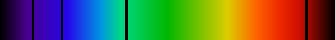
\includegraphics[scale = 0.45]{Figures/absorption.png}
         \caption{Absorption lines (discrete spectrum)}
         \label{fig:five over x}
     \end{subfigure}
        \caption{Visualising various spectra}
        \label{fig:three graphs}
    \end{figure}
    \par
    Spectral lines can be influenced in the presence of electric (\textit{Stark effect}) and magnetic fields (\textit{Zeeman effect}).
    \par
    In 1896, shortly before moving from Leiden to Amsterdam, Dutch physicist Pieter Zeeman discovered that a spectral line is split into several components in the presence of a magnetic field. Fellow physicist Hendrik Lorentz heard about Zeeman's observations at the meeting of the Royal Netherlands Academy of Arts and Sciences in Amsterdam, where these results were communicated by Kamerlingh Onnes. Lorentz called Zeeman into his office and presented him with an explanation of his observations, based on Lorentz's theory of electromagnetic radiation. Zeeman's discovery had confirmed Lorentz's prediction about the polarization of light emitted in the presence of a magnetic field. Thanks to Zeeman's work it became clear that the oscillating particles that according to Lorentz were the source of light emission were negatively charged, and were a thousandfold lighter than the hydrogen atom. This conclusion was reached well before J. J. Thomson's discovery of the electron. The Zeeman effect thus became an important tool for elucidating the structure of the atom. Zeeman was awarded the 1902 Nobel Prize in Physics for his discovery. 
    \par
    Zeeman effect is analogous to Stark effect and transitions between different components have, in general, different intensities, with some being entirely forbidden (in the dipole approximation), as governed by the selection rules.
    \par
    Since the distance between the Zeeman sub-levels is a function of magnetic field strength, this effect can be used to measure magnetic field strength, e.g. that of the Sun and other stars or in laboratory plasmas. The Zeeman effect is very important in applications such as nuclear magnetic resonance spectroscopy, electron spin resonance spectroscopy, magnetic resonance imaging (MRI) and Mössbauer spectroscopy\footnote{a spectroscopy technique based on the resonant and recoil-free emission and absorption of gamma radiation by atomic nuclei bound in a solid.}. It may also be utilized to improve accuracy in atomic absorption spectroscopy. A theory about the magnetic sense of birds assumes that a protein in the retina is changed due to the Zeeman effect.
    \begin{figure}
        \centering
        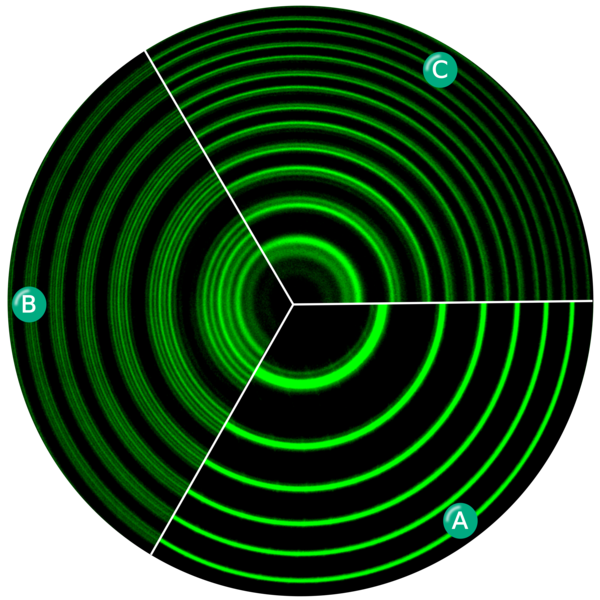
\includegraphics[scale = 0.75]{Figures/zeemanillus.png}
        \caption{The spectral lines of mercury vapor lamp at wavelength 546.1 nm, showing anomalous Zeeman effect. (A) Without magnetic field. (B) With magnetic field, spectral lines split as transverse Zeeman effect. (C) With magnetic field, split as longitudinal Zeeman effect. The spectral lines were obtained using a Fabry–Pérot interferometer.}
        \label{fig:illus}
    \end{figure}
    
\section{Theory}
    The phenomena discovered by Zeeman in 1896 is now retrospectively called \textit{normal} Zeeman effect. In 1898, Thomas Preston observed quartet pattern of lines in a magnetic field which is now referred to as the \textit{anomalous} Zeeman effect.
    \par
    Consider an external magnetic field $\mathbf{B}$ (figure (\ref{fig:torque})), a magnetic dipole has an amount of potential energy $U_m$ that depends upon both the magnitude of its magnetic moment and the orientation of this moment with respect to the field.
    \begin{figure}
        \centering
        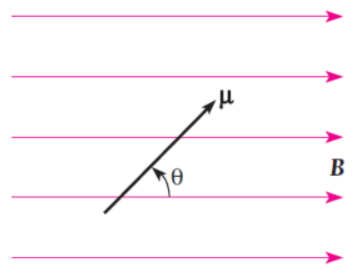
\includegraphics[scale = 0.8]{Figures/torque.png}
        \caption{Torque on a magnetic dipole}
        \label{fig:torque}
    \end{figure}
    The torque on a magnetic dipole in a magnetic field of flux density $\mathbf{B}$ is
    \begin{equation}
        \tau = \mu B \sin \theta 
    \end{equation}
    If we take $U_m = 0$ when $\theta = \pi / 2 = 90 \degree$,
    \begin{equation}
        U_m = \int_{\pi/2}^{\theta} \tau d \theta = \mu B \int_{\pi/2}^{\theta} \sin \theta d \theta = - \mu B \cos \theta
    \end{equation}
    The magnetic moment of the orbital electron in an atom depends on its angular momentum $\mathbf{L}$. By taking the current loop formulation we can write,
    \begin{equation}
        \mathbf{\mu} = - \Big( \dfrac{e}{2m}\Big) \mathbf{L}
    \end{equation}
    So the magnetic energy can be written as,
    \begin{equation}
        U_m = \Big( \dfrac{e}{2m}\Big) LB \cos \theta
    \end{equation}
    As we know the angle $\theta$ between the $\mathbf{L}$ and $z$ direction can only, we have, 
    \begin{equation}
        \cos \theta = \dfrac{m_l}{\sqrt{l(l+1)}}
    \end{equation}
    and
    \begin{equation}
        L = \sqrt{l(l+1)} \hbar
    \end{equation}
    We rewrite magnetic energy as
    \begin{equation}
        U_m = m_l \mu_B B
    \end{equation}
    where $\mu_B = \dfrac{e \hbar}{2m}$ is the Bohr magneton which will be later determined in the experiment.
    \par
    Let's first consider the normal Zeeman effect (figure (\ref{fig:normalzeeman})). since the magnetic quantum number $m_l$ can have the $2l+1$ values of $l$ through $0$ to $l$, a state of given orbital quantum number $l$ splits into $2l+1$ sub-states that differ in energy by $\mu_B B$ when the atom is in a magnetic field. The selection rule only allow changes $\Delta m = 0, \pm -1$. So we expect a spectral line from a transition between two states of different $l$ to be split into only three components:
    \begin{equation}
        \begin{split}
            \nu_1
            &= \nu_0 - \mu_B \dfrac{B}{h} = \nu_0 - \dfrac{e}{4 \pi m} B \\
            \nu_2
            &= \nu_0 \\
            \nu_3
            &= \nu_0 + \mu_B \dfrac{B}{h} = \nu_0 + \dfrac{e}{4 \pi m} B
        \end{split}
    \end{equation}
    So we will get a single spectral line splits into there in presence of magnetic field. The amount of splitting depends on the strength of magnetic field, which we will verify in this experiment.
    \begin{figure}
        \centering
        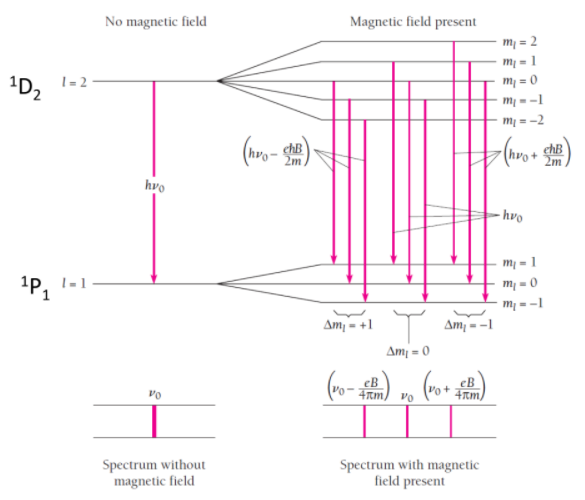
\includegraphics[scale = 0.62]{Figures/normalzeeman.png}
        \caption{Normal Zeeman effect}
        \label{fig:normalzeeman}
    \end{figure}
    \par
    The anomalous Zeeman effect is the more general case where the electron spins do not cancel each other and the energy of an atomic state in a magnetic field depends on both the magnetic moments of electron orbit and electron spin. The spin moment can be written as,
    \begin{equation}
        \Vec{\mu_S} = - \Big( \dfrac{e}{2 m_e} \Big) \Vec{S} = -g_S \mu_B \dfrac{\Vec{S}}{\hbar}
    \end{equation}
    As $\abs{\Vec{S}} = \hbar \sqrt{s(s+1)}$, we have
    \begin{equation}
        \mu_S = \abs{-g_s \mu_B \sqrt{s(s+1)}}
    \end{equation}
    Since the spin and orbital angular moment are coupled ($L-S$ coupling), the total angular moment can be written as
    \begin{equation}
        \abs{\Vec{J}} = \abs{\Vec{L} + \Vec{S}} = \hbar \sqrt{J(J+1)}
    \end{equation}
    The gyromagnetic ratio, which is 1 for pure orbital and 2 for pure spin case, becomes
    \begin{equation}
        g_J = 1 + \dfrac{J(J+1) + S(S+1) - L(L+1)}{2J(J+1)}
    \end{equation}
    The magnetic quantum number $m_J$ will change from $J, J-1, \ldots, -J$. The magnetic energy becomes
    \begin{equation}
        U_{mJ} = -m_J g_J \mu_B B_0
    \end{equation}
    For the anomalous Zeeman effect the used transition in Cd is from $^3S_1$ to $^3P_2$. The superscript (here 3) represents multiplicity, i.e. $2s+1$, the subscript represents $J = l+s$. Thus, The energy difference between the initial sub-states in magnetic field ($^3S_1$) is $\Delta E = -2 \mu_B B_0$ and The energy difference between the final sub-states in magnetic field ($^3P_2$) is $\Delta E = -1.5 \mu_B B_0$. The selection rules remain the same.
    \par
    The splitting of the Cd-spectral line $l = \SI{643.8}{\nano \metre}$ into three lines, the so-called Lorentz triplets, occurs since the Cd-atom represents a singlet system of total spin $S= 0$. In the absence of a magnetic field there is only one possible $D \rightarrow P$ transition of $\SI{643.8}{\nano \metre}$, as indicated by figure (\ref{fig:splitting})
    \begin{figure}
        \centering
        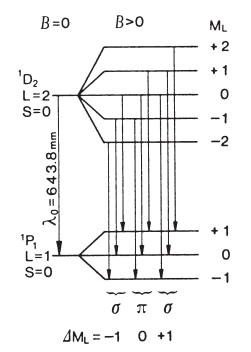
\includegraphics{Figures/splitting.png}
        \caption{Splitting up of the components in the magnetic field and permitted transitions.}
        \label{fig:splitting}
    \end{figure}
    In the presence of a magnetic field the associated energy levels split into $2l+1$ components. Radiating transitions between these components are possible, provided that the selection rules mentioned earlier are taken into account. In this case, therefore, there are a total of nine permitted transitions. These nine transitions can be grouped into three groups of three transitions each, where all transitions in a group have the same energy and hence the same wavelength. Therefore, only three lines will be visible.
    \par
    The first group where $\Delta m_l = -1$ gives a $\sigma$-line the light of which is polarized vertically to the magnetic field. The middle group $\Delta m_l = 0$ gives a $\pi$-line. This light is polarized parallel to the direction of the field. The last group where $\Delta m_l = +1$ gives a $\sigma$-line the light of which is again polarized vertically to the magnetic field.
    \par
    In the absence of the analyser all three lines can be seen simultaneously. Each ring which was observed in the absence of a magnetic field is split into three rings when a magnetic field is applied. Inserting the analyser the two $\sigma$-lines can be observed exclusively if the analyser is in the vertical position, while only the $\pi$-line appears if the analyser is turned into its horizontal position (\textit{transverse Zeeman effect}). Turning the electromagnet by $90 \degree$ the light coming from the spectral lamp parallel to the direction of the field can also be studied since the pole-shoes have been drilled. It can be shown that this light is circular polarized light. Whatever the position of the analyser may be, each of the rings seen without a magnetic field is now permanently split into two rings in the presence of a magnetic field (\textit{longitudinal Zeeman effect}). Figure (\ref{fig:long}) summarizes the facts.
    \begin{figure}
        \centering
        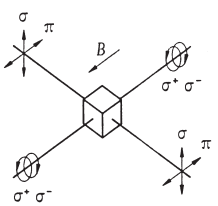
\includegraphics{Figures/longtranszeeman.png}
        \caption{Longitudinal and transverse Zeeman effect.}
        \label{fig:long}
    \end{figure}
    Turning the electromagnet back for the observation of the two $\sigma$-lines of the transverse Zeeman effect it is easy to see that the size of the splitting increases with increasing magnetic field strength. For a quantitative measurement of this splitting in terms of number of wavelengths, a Fabry-Perot interferometer is used, the functioning of which may briefly be explained. The Fabry-Perot étalon has a resolution of approximately 300000. That means that a wavelength change of approximately 0.002 nm can still be detected.
    \begin{figure}
        \centering
        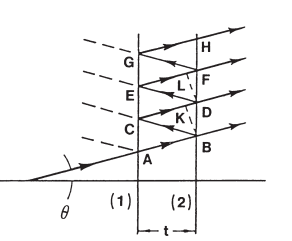
\includegraphics{Figures/reflec.png}
        \caption{Reflected and transmitted rays at the parallel surfaces (1) and (2) of the étalon. The étalon spacing is $t$.}
        \label{fig:reflec}
    \end{figure}
    \par 
    The étalon consists of two parallel flat glass plates coated on the inner surface with a partially reflecting layer. Let us consider the two partially transmitting surfaces (1) and (2) in figure (\ref{fig:reflec}) separated by a distance $t$. An incoming ray forming an angle $\theta$ with the normal to the plates will be split into the rays $AB$, $CD$, $EF$, etc. the path difference between the wave fronts of two adjacent rays (for example, $AB$ and $CD$) is
    \begin{equation}
        \delta = BC + CK
    \end{equation}
    where, obviously, BK is normal to CD. With
    \begin{equation}
        CK = BC \cos 2 \theta; BC \cos \theta = t
    \end{equation}
    From here we obtain
    \begin{equation}
        \begin{split}
            \delta = BCK
            &= BC (1 + \cos 2 \theta) \\
            &= 2 BC \cos^2 \theta \\
            &= 2 t \cos \theta
        \end{split}
    \end{equation}
    and for a constructive interference to occur one must demand:
    \begin{equation}
        n \lambda = 2 t \cos \theta
    \end{equation}
    $n$ being an integer. Taking account the refractive index in account, we have
    \begin{equation}
    \label{eq1}
        n \lambda = 2 \mu t \cos \theta
    \end{equation}
    Equation (\ref{eq1}) is the basic interferometer equation. Let the parallel rays $B$, $D$, $F$ etc. be brought to a focus by the use of a lens of focal length $f$ as shown in figure (\ref{fig:focus}).
    \begin{figure}
        \centering
        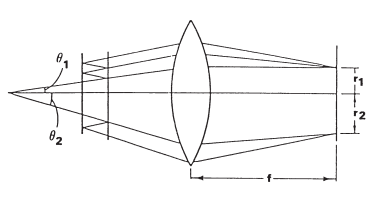
\includegraphics{Figures/focus.png}
        \caption{Focusing of the light emerging from a Fabry-Perot étalon. Light entering the étalon at an angle $\theta$ is focused onto a ring of radius $r = f \theta$ where $f$ is the focal length of the lens.}
        \label{fig:focus}
    \end{figure}
    Then, $\theta$ fulfills equation (\ref{eq1}), bright rings will appear in the focal plane, their radius being given by
    \begin{equation}
        r_n = f \tan \theta_n \simeq f \theta_n
    \end{equation}
    Upon solving using equations derived earlier, we obtain
    \begin{equation}
        \theta_n = \sqrt{\dfrac{2(n_0 - n)}{n_0}}
    \end{equation}
     If $n_1$ is the interference order of the first ring, clearly $n_1 > n_0$ since $n_1 = n_0 \cos \theta_{n_1}$. We then let
    \begin{equation}
        n_1 = n_0 - \varepsilon; 0 < \varepsilon < 1
    \end{equation}
    where $n_1$ is the closest integer to $n_0$ (smaller than $N_0$). Thus, we have in general for the $p$-th ring of the pattern, as measured from the center out,
    \begin{equation}
        n_p = (n_0 - \varepsilon) - (p-1)
    \end{equation}
    From here we obtain
    \begin{equation}
        r_{p+1}^2 - r_p^2 = \dfrac{2f^2}{n_0}
    \end{equation}
    Now, if there are two components of a spectral line (splitting of one central line into two components) with wavelengths $\lambda_a$ and $\lambda_b$, which are very close to one another, they will have fractional orders at the center $\varepsilon_a$ and $\varepsilon_b$:
    \begin{equation}
        \begin{split}
            \varepsilon_a
            &= \dfrac{2 \mu t}{\lambda_a} - n_{1, a} = 2 \mu t \Bar{\nu_a} - n_{1, a} \\
            \varepsilon_b
            &= \dfrac{2 \mu t}{\lambda_b} - n_{1, b} = 2 \mu t \Bar{\nu_b} - n_{1, b}
        \end{split}
    \end{equation}
    where $n_{1, a}$, $n_{1, b}$ is the interference order of the first ring. The difference in the wave numbers thus is
    \begin{equation}
        \Delta \Bar{\nu} = \Bar{\nu_a} - \Bar{\nu_b} = \dfrac{\varepsilon_a - \varepsilon_b}{2 \mu t}
    \end{equation}
    The final equation for $\Delta \Bar{\nu}$ we get is
    \begin{equation}
        \Delta \Bar{\nu} = \dfrac{1}{2 \mu t} \Bigg( \dfrac{r_{p+1, a}^2}{r_{p+1, a}^2 - r_{p, a}^2} - \dfrac{r_{p+1, b}^2}{r_{p+1, b}^2 - r_{p, b}^2} \Bigg)
    \end{equation}
    Rewriting this after taking $\delta_{a, b}^{p+1, p} = r_{p+1, a}^2 - r_{p+1, b}^2$ and $\Delta_a^{p+1, p} = \Delta_b^{p+1, p}$ we finally get our working formula as
    \begin{equation}
        \boxed{\Delta \Bar{\nu} = \dfrac{1}{2 \mu t} \dfrac{\delta}{\Delta}}
    \end{equation}
    The difference in wave numbers of one of the $\sigma$-lines with respect to the central lines is $\Delta \Bar{\nu}/2$. For the radiating electrons this means, for instance, a change in energy of
    \begin{equation}
        \Delta E = hc \dfrac{\Delta \Bar{\nu}}{2}
    \end{equation}
    On the other hand the change in energy $\Delta E$ is proportional to the magnetic flux density $B$. The factor of proportionality between $\Delta E$ and $B$ is the Bohr magneton. Thus
    \begin{equation}
    \label{eqbohr}
        \boxed{\mu_B = hc \dfrac{\Delta \Bar{\nu}}{2B}}
    \end{equation}
    
\section{Experimental Set-up and Procedure}
    The experimental set-up of the experiment is presented in figure (\ref{fig:cmos}).
    \begin{figure}
        \centering
        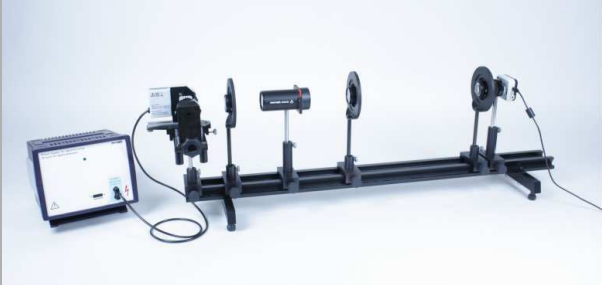
\includegraphics[scale = 0.6]{Figures/cmossetup.png}
        \caption{Experimental setup	with CMOS-camera}
        \label{fig:cmos}
    \end{figure}
    The electromagnet is put on the rotating table for heavy loads and mounted with the two pole-shoes with holes in such a way that a gap large enough for the Cd-lamp (9-11 mm) remains for the Cd-lamp. The pole-shoes have to be well tightened in such a way that they cannot move later on when the magnetic flux is established. The Cd-lamp is inserted into the gap without touching the pole-shoes and connected to the power supply for spectral lamps. The coils of the electromagnet are connected in parallel and via an ammeter connected to the variable power supply of up to 20 VDC, 12 A. A capacitor of $\SI{22000}{\micro \farad}$ is in parallel to the power output to smoothen the DC-voltage.
    \par
    The optical bench for investigation of the line splitting carries the following elements (their approximate position in cm is given in brackets) and is illustrated in figure (\ref{fig:optical}):
    \begin{itemize}
        \item (80) CMOS Camera
        \item (73) $L_3 = \SI{50}{\milli \metre}$
        \item (68) Screen with scale
        \item (45) Analyser
        \item (39) $L_3 = \SI{300}{\milli \metre}$
        \item (33) Fabry-Perot Etalon
        \item (25) $L_3 = \SI{50}{\milli \metre}$
        \item (20) Iris diaphragm
        \item (20) Drilled pole-shoes
        \item Cd-spectral lamp on rotating table
    \end{itemize}
    \begin{figure*}
        \centering
        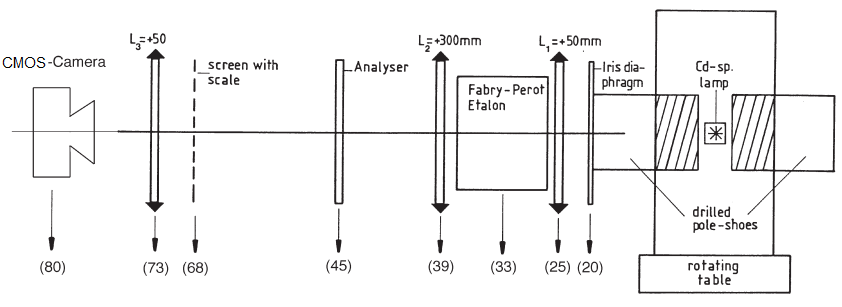
\includegraphics{Figures/optical arrangement.png}
        \caption{Arrangement of the optical components.}
        \label{fig:optical}
    \end{figure*}
    The iris diaphragm is eliminated for initial adjustment and for the observation of the longitudinal Zeeman effect. During observation of the transverse Zeeman effect the iris diaphragm is illuminated by the Cd-lamp and such it acts as the light source. The lens $L_1$ and a lens of $f = \SI{100}{\milli \metre}$, incorporated in the étalon, create a nearly parallel light beam which the Fabry-Perot étalon needs for a proper interference pattern.
    \par
    The etalon contains a removable colour filter that lets the red cadmium line at $\SI{643.8}{\nano \metre}$ pass. The lens $L_2$ produces an interference pattern of rings which can be observed through L3. The ring diameters can be measured using the CMOS-camera and the software supplied with it. In the classical version the interference pattern is produced within the plane of the screen with a scale mounted on a slide mount which can laterally be displaced with a precision of 1/100th of a millimeter. The measurement here can be done for instance, by systematic displacement of the slash representing the `0' of the scale.
    \par
    The initial adjustment is done in the following way: The rotating table with electromagnet, pole-shoes and Cd-lamp already mounted is adjusted so that the center of the holes in the pole-shoes lies about 28 cm above the table. The optical bench with all elements (except iris diaphragm and CMOS-camera) mounted, is then moved closer to the electromagnet in such a way that one of the outlet holes of the pole-shoes coincides with the previous position of the iris diaphragm. $L_1$ is then adjusted so that the outlet hole is within the focal plane of it. All other optical elements of figure (\ref{fig:optical}). are subsequently readjusted with respect to their height correspondingly. The current of the coils is set for some time to 8 A (increase in light intensity of the Cd-lamp) and the ring interference pattern in axial direction is observed through $L_3$ by the eye. The pattern must be centered and sharp which is eventually achieved by a last, slight movement of the étalon (to the right or to the left) and by displacement of $L_2$ (vertically and horizontally).
    \par
    Finally the CMOS-camera with the 8 mm lens attached is mounted to the optical bench and adjusted in horizontal and vertical position as well as in tilt and focus until a clear picture of the ring pattern is visible on the computer screen. The electromagnet is now turned by $90 \degree$, the iris diaphragm is inserted and the analyzer turned until the $\pi$-line disappears completely and the two $\sigma$-lines appear clearly visible.

    

\section{Observations}
    The make of the instrument is PHYWE.
    \begin{enumerate}
        \item The refractive index at $\lambda = \SI{643.8}{\nano \metre}$, $\mu = 1.456$
        \item The etalon spacing, $t = \SI{3}{\milli \metre}$
    \end{enumerate}
    \begin{table}[]
    \centering
    \caption{Readings for the experiment}
    \label{tab:data}
    \begin{tabular}{@{}cccccc@{}}
    \toprule
    \begin{tabular}[c]{@{}c@{}}\textbf{Distance}\\ (mm)\end{tabular} & \begin{tabular}[c]{@{}c@{}}\textbf{Order of fringe}\\ $p$\end{tabular} & \begin{tabular}[c]{@{}c@{}}$r_a$\\ ($\mu$ m)\end{tabular} & \begin{tabular}[c]{@{}c@{}}$r_b$\\ ($\mu$ m)\end{tabular} & \begin{tabular}[c]{@{}c@{}}$B$\\ (mT)\end{tabular} & \begin{tabular}[c]{@{}c@{}}$\Delta \Bar{\nu}$\\ ($m^{-1}$)\end{tabular} \\ \midrule
        40                                             & 1                                                 & 18.97                                             & 66.955                                            & \multirow{3}{*}{580}                             & \multirow{3}{*}{59.56687}                           \\
    40                                             & 2                                                 & 89.26                                             & 110.47                                            &                                                  &                                                     \\
    40                                             & 3                                                 & 127.09                                            & 141.49                                            &                                                  &                                                     \\
    42                                             & 1                                                 & 28.865                                            & 62.715                                            & \multirow{3}{*}{450}                             & \multirow{3}{*}{49.0555}                            \\
    42                                             & 2                                                 & 92.45                                             & 108.1                                             &                                                  &                                                     \\
    42                                             & 3                                                 & 126.51                                            & 140.41                                            &                                                  &                                                     \\
    44                                             & 1                                                 & 33.395                                            & 60.045                                            & \multirow{3}{*}{360}                             & \multirow{3}{*}{39.84824}                           \\
    44                                             & 2                                                 & 94.46                                             & 106.96                                            &                                                  &                                                     \\
    44                                             & 3                                                 & 128.12                                            & 139.89                                            &                                                  &                                                     \\
    46                                             & 1                                                 & 36.31                                             & 57.39                                             & \multirow{2}{*}{290}                             & \multirow{2}{*}{31.60394}                           \\
    46                                             & 2                                                 & 93.91                                             & 105.16                                            &                                                  &                                                     \\ \bottomrule
    \end{tabular}
    \end{table}
    The graph between $B$ and $\Delta \Bar{\nu}$ from data in table (\ref{tab:data}) is plotted in figure (\ref{fig:plot-1}).
    \begin{figure}
        \centering
        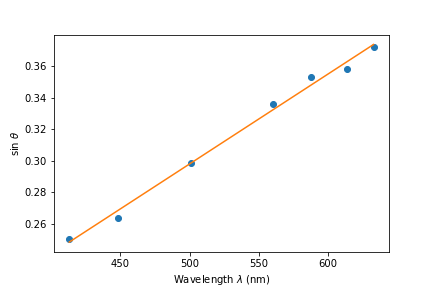
\includegraphics[scale = 0.56]{Figures/plot-1.png}
        \caption{The $B \sim \Delta \Bar{\nu}$ plot}
        \label{fig:plot-1}
    \end{figure}

\section{Calculations and Results}
    Now the Bohr magneton is given from (\ref{eqbohr}) as
    \begin{equation}
    \label{eq26}
        \mu_B = \dfrac{hc}{2} m_{slope}
    \end{equation}
    where $m_{slope}$ is the slope of the line plotted in figure (\ref{fig:plot-1}).
    The five summations of for the data set plotted in figure (\ref{fig:plot-1}) are as follows:
    \par
    \vspace{0.5cm}
    $S_{x} = \mathlarger{\mathlarger{\sum}} x_{i} = \SI{1680}{\milli \tesla}$, \hspace{0.25cm} $S_{y} = \mathlarger{\mathlarger{\sum}} y_{i} = \SI{180.074}{\per \metre}$,
    \par
    \vspace{0.5cm}
    $S_{xx} = \mathlarger{\mathlarger{\sum}} x_{i}^2 = \SI{752600}{\milli \tesla \squared}$,
    \par
    \vspace{0.5cm}
    $S_{yy} = \mathlarger{\mathlarger{\sum}} y_{i}^2 = \SI{8541.344518}{\per \metre \squared}$,
    \par
    \vspace{0.5cm}
    $S_{xy} = \mathlarger{\mathlarger{\sum}} x_{i}y_{i} = \SI{80134.26488}{\milli \tesla \per \metre}$.
    \par
    \vspace{0.5cm}
    Now the slope is given by,
    \begin{equation}
        m_{\nu_1} = \dfrac{S S_{xy} - S_{x}S_{y}}{S S_{xx} - S_{x}^2} = \SI{95.8076}{\per \metre \per \tesla}
    \end{equation}
    Now, putting in the values in (\ref{eq26}), we get 
        \begin{equation}
            \boxed{\mu_B = \SI{9.522e-24}{\joule \per \tesla}} 
        \end{equation}
    
    

\section{Error Analysis}
    Error in $\mu_B$ is equal to the error in slope as rest terms are assumed exact. Now error in slope is given by
    \begin{equation}
    \label{eqslope}
        \sigma_m = \sigma_y \times \sqrt{\dfrac{S}{\Delta}}
    \end{equation}
    $\sigma_y$ is the uncertainty in the measurement of $\Delta \Bar{\nu}$. We need uncertainties in $\delta$ and $\Delta$ to calculate that. Using propagational error forumale, we obtain $d m_{slope} = \SI{5.241}{\per \metre \per \tesla}$ (considering the maximum error). Putting in the values in equations (\ref{eqslope}) and solving, we get
    \begin{equation}
        \boxed{d \mu_{B} = \SI{1.041e-24}{\joule \per \tesla}}
    \end{equation}


        

\section{Discussions}
\begin{enumerate}
    \item the effect is demonstrated with the light of a Cadmium lamp and the help of a Fabry-Perot interferometer for resolving a small part of the spectrum pre-selected by a color filter or an interference filter so only the light of a single atomic transition line is observed.
    \item Without field the magnetic sub-levels have the same energy but with field the degeneration of the levels with different is cancelled and the line is split.
    \item Cadmium has a similar outer electron structure to that of Helium but also of Mercury. In a completed shell in it's ground state the electron spins always compensate each other – they are anti-parallel. If the total electron spin is zero, also the magnetic moment connected to electron spin is zero. Atomic states with zero total spin are called singlet states. So in transitions between different singlet states the magnetic moment of spin does not play a role, as is the case with the normal Zeeman effect.
    \item The $B \sim \Delta \Bar{\nu}$ plot was obtained to be a straight line, that is, with increase in magnetic field, the difference in wave numbers increased.
\end{enumerate}



\section{Conclusions}
\begin{enumerate}
    \item The value of $\mu_B$ was found to be $\mu_B = \SI[separate-uncertainty=true]{9 \pm 1e-24}{\joule \per \tesla}$ after taking care of the significant figures.
    \item The results so obtained were in close to the literature value. The experiment was thus a success.
\end{enumerate}




% Produces the bibliography via BibTeX.

\end{document}
%
% ****** End of file apssamp.tex ******
